\documentclass[11pt,a4paper]{article}
\usepackage{graphicx}
\usepackage{tcolorbox}
\usepackage{xcolor}
\usepackage{geometry}
\usepackage{tikz}
\usepackage{amsmath}
\usepackage{amssymb}
\usetikzlibrary{calc,arrows.meta,patterns}
\geometry{margin=0.8in}

% Define colors
\definecolor{mlblue}{RGB}{31, 119, 180}
\definecolor{mlorange}{RGB}{255, 127, 14}
\definecolor{mlgreen}{RGB}{44, 160, 44}
\definecolor{mlred}{RGB}{214, 39, 40}
\definecolor{mlpurple}{RGB}{148, 103, 189}
\definecolor{mlyellow}{RGB}{241, 196, 15}
\definecolor{mlcyan}{RGB}{23, 190, 207}
\definecolor{mlgray}{RGB}{150, 150, 150}

\title{\Large\textbf{Advanced Discovery: DBSCAN Algorithm}\\
\vspace{0.3em}
\normalsize Density-Based Spatial Clustering of Applications with Noise}
\date{}

\begin{document}
\maketitle
\vspace{-2em}

\section*{Core Concept: Density = Connectivity}

\begin{center}
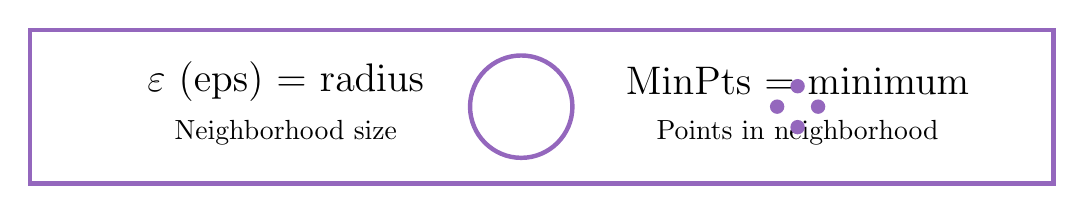
\begin{tikzpicture}[scale=1.3]
% Two key parameters
\draw[ultra thick, mlpurple] (0,0) rectangle (10,1.5);
\node at (2.5,1) {\Large $\varepsilon$ (eps) = radius};
\node at (2.5,0.5) {Neighborhood size};
\draw[mlpurple, ultra thick] (4.8,0.75) circle (0.5);

\node at (7.5,1) {\Large MinPts = minimum};
\node at (7.5,0.5) {Points in neighborhood};
\foreach \i in {1,...,4} {
    \fill[mlpurple] (7.5,0.75) ++(90*\i:0.2) circle (2pt);
}
\end{tikzpicture}
\end{center}

\vspace{0.5em}

\section*{Three Types of Points}

\begin{center}
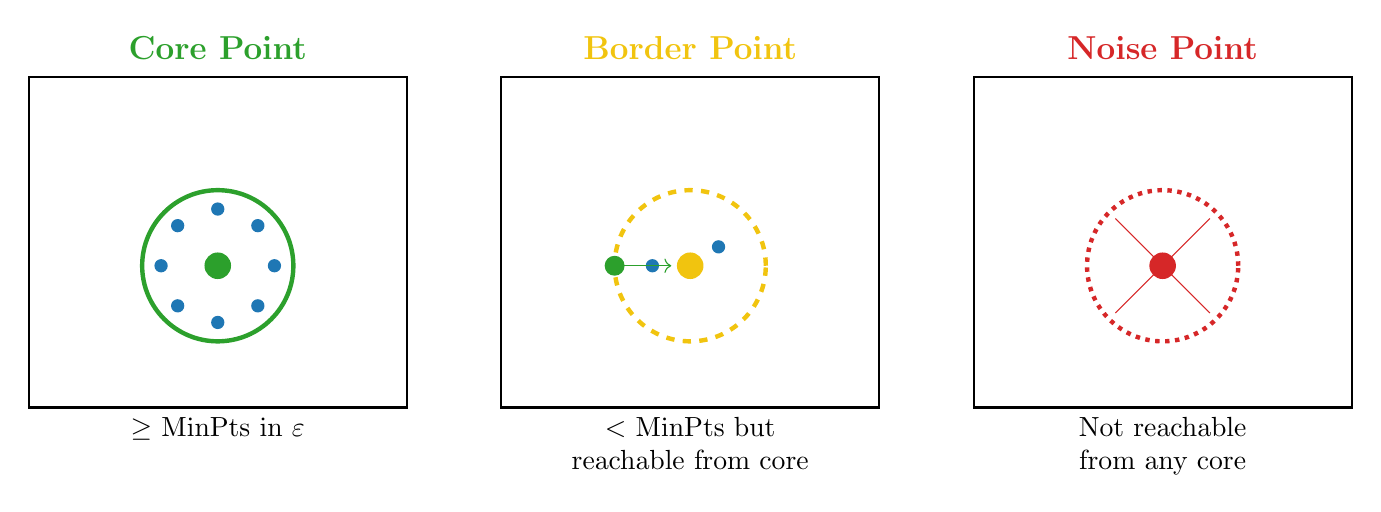
\begin{tikzpicture}[scale=1.2]
% Core point
\begin{scope}[shift={(0,0)}]
\draw[thick] (0,0) rectangle (4,3.5);
\node[font=\large\bfseries, mlgreen] at (2,3.8) {Core Point};

% Central core point
\fill[mlgreen] (2,1.5) circle (4pt);
\draw[mlgreen, ultra thick] (2,1.5) circle (0.8);
\node[mlgreen] at (2,1.5) {C};

% Neighbors (>= MinPts in eps)
\foreach \angle in {0,45,90,135,180,225,270,315} {
    \fill[mlblue] (2,1.5) ++(\angle:0.6) circle (2pt);
}
\node[below] at (2,0) {$\geq$ MinPts in $\varepsilon$};
\end{scope}

% Border point
\begin{scope}[shift={(5,0)}]
\draw[thick] (0,0) rectangle (4,3.5);
\node[font=\large\bfseries, mlyellow] at (2,3.8) {Border Point};

% Border point
\fill[mlyellow] (2,1.5) circle (4pt);
\draw[mlyellow, ultra thick, dashed] (2,1.5) circle (0.8);
\node[mlyellow] at (2,1.5) {B};

% Few neighbors
\fill[mlblue] (1.6,1.5) circle (2pt);
\fill[mlblue] (2.3,1.7) circle (2pt);
\fill[mlgreen] (1.2,1.5) circle (3pt);
\draw[mlgreen, ->] (1.2,1.5) -- (1.8,1.5);

\node[below, align=center] at (2,0) {$<$ MinPts but\\reachable from core};
\end{scope}

% Noise point
\begin{scope}[shift={(10,0)}]
\draw[thick] (0,0) rectangle (4,3.5);
\node[font=\large\bfseries, mlred] at (2,3.8) {Noise Point};

% Isolated point
\fill[mlred] (2,1.5) circle (4pt);
\draw[mlred, ultra thick, dotted] (2,1.5) circle (0.8);
\node[mlred] at (2,1.5) {N};
\draw[mlred] (1.5,1) -- (2.5,2);
\draw[mlred] (1.5,2) -- (2.5,1);

\node[below, align=center] at (2,0) {Not reachable\\from any core};
\end{scope}
\end{tikzpicture}
\end{center}

\vspace{0.5em}

\section*{DBSCAN vs K-Means: Shape Discovery}

\begin{center}
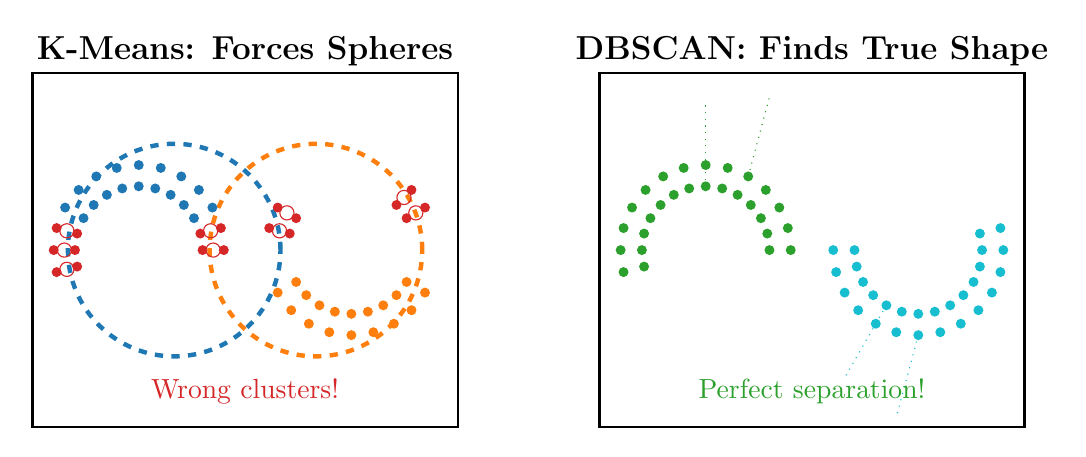
\begin{tikzpicture}[scale=0.9]
% K-means result
\begin{scope}[shift={(0,0)}]
\draw[thick] (0,0) rectangle (6,5);
\node[font=\large\bfseries] at (3,5.3) {K-Means: Forces Spheres};

% Draw two crescents poorly separated
\draw[mlblue, ultra thick, dashed] (2,2.5) circle (1.5);
\draw[mlorange, ultra thick, dashed] (4,2.5) circle (1.5);

% Crescent data points
\foreach \angle in {30,45,60,75,90,105,120,135,150} {
    \fill[mlblue] (1.5,2.5) ++(\angle:1.2) circle (2pt);
    \fill[mlblue] (1.5,2.5) ++(\angle:0.9) circle (2pt);
}
\foreach \angle in {210,225,240,255,270,285,300,315,330} {
    \fill[mlorange] (4.5,2.5) ++(\angle:1.2) circle (2pt);
    \fill[mlorange] (4.5,2.5) ++(\angle:0.9) circle (2pt);
}

% Misclassified points
\foreach \angle in {0,15,165,180,195} {
    \fill[mlred] (1.5,2.5) ++(\angle:1.2) circle (2pt);
    \fill[mlred] (1.5,2.5) ++(\angle:0.9) circle (2pt);
    \draw[mlred] (1.5,2.5) ++(\angle:1.05) circle (0.1);
}
\foreach \angle in {30,45,150,165} {
    \fill[mlred] (4.5,2.5) ++(\angle:1.2) circle (2pt);
    \fill[mlred] (4.5,2.5) ++(\angle:0.9) circle (2pt);
    \draw[mlred] (4.5,2.5) ++(\angle:1.05) circle (0.1);
}

\node[mlred] at (3,0.5) {Wrong clusters!};
\end{scope}

% DBSCAN result
\begin{scope}[shift={(8,0)}]
\draw[thick] (0,0) rectangle (6,5);
\node[font=\large\bfseries] at (3,5.3) {DBSCAN: Finds True Shape};

% Correctly identified crescents
\foreach \angle in {0,15,30,45,60,75,90,105,120,135,150,165,180,195} {
    \fill[mlgreen] (1.5,2.5) ++(\angle:1.2) circle (2pt);
    \fill[mlgreen] (1.5,2.5) ++(\angle:0.9) circle (2pt);
}
\foreach \angle in {180,195,210,225,240,255,270,285,300,315,330,345,360,15} {
    \fill[mlcyan] (4.5,2.5) ++(\angle:1.2) circle (2pt);
    \fill[mlcyan] (4.5,2.5) ++(\angle:0.9) circle (2pt);
}

% Show density connections
\draw[mlgreen, dotted] (1.5,2.5) ++(60:1.2) -- ++(75:1.2);
\draw[mlgreen, dotted] (1.5,2.5) ++(90:0.9) -- ++(90:1.2);
\draw[mlcyan, dotted] (4.5,2.5) ++(270:1.2) -- ++(255:1.2);
\draw[mlcyan, dotted] (4.5,2.5) ++(240:0.9) -- ++(240:1.2);

\node[mlgreen] at (3,0.5) {Perfect separation!};
\end{scope}
\end{tikzpicture}
\end{center}

\newpage

\section*{Algorithm Flow: Growing Clusters}

\begin{center}
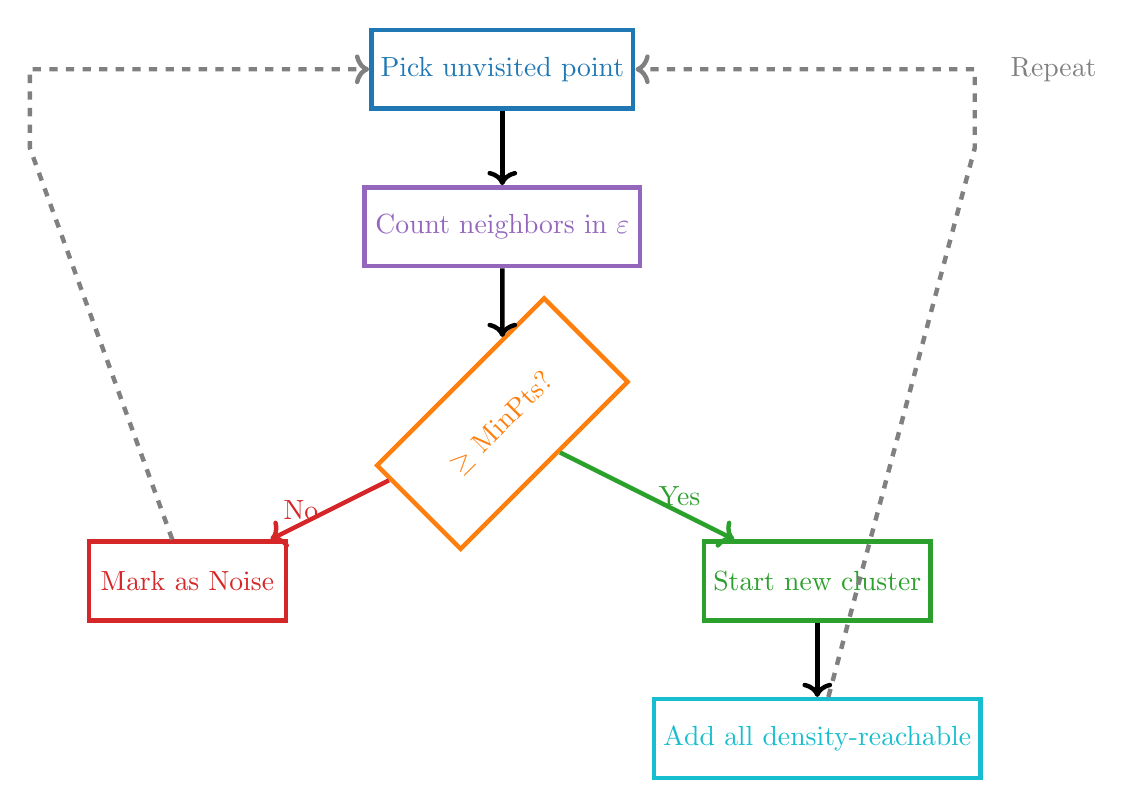
\begin{tikzpicture}[scale=1]
% Step 1
\node[draw, ultra thick, mlblue, minimum width=3cm, minimum height=1cm] (start) at (0,0) {Pick unvisited point};

% Step 2
\node[draw, ultra thick, mlpurple, minimum width=3.5cm, minimum height=1cm] (check) at (0,-2) {Count neighbors in $\varepsilon$};

% Decision
\node[draw, ultra thick, mlorange, minimum width=3cm, minimum height=1.5cm, rotate=45] (decide) at (0,-4.5) {$\geq$ MinPts?};

% Noise path
\node[draw, ultra thick, mlred, minimum width=2.5cm, minimum height=1cm] (noise) at (-4,-6.5) {Mark as Noise};

% Core path
\node[draw, ultra thick, mlgreen, minimum width=2.5cm, minimum height=1cm] (core) at (4,-6.5) {Start new cluster};

% Expand
\node[draw, ultra thick, mlcyan, minimum width=3.5cm, minimum height=1cm] (expand) at (4,-8.5) {Add all density-reachable};

% Arrows
\draw[->, ultra thick] (start) -- (check);
\draw[->, ultra thick] (check) -- (decide);
\draw[->, ultra thick, mlred] (decide) -- node[left] {No} (noise);
\draw[->, ultra thick, mlgreen] (decide) -- node[right] {Yes} (core);
\draw[->, ultra thick] (core) -- (expand);

% Loop back
\draw[->, ultra thick, gray, dashed] (noise) -- (-6,-1) -- (-6,0) -- (start);
\draw[->, ultra thick, gray, dashed] (expand) -- (6,-1) -- (6,0) -- (start);

\node[gray] at (7,0) {Repeat};
\end{tikzpicture}
\end{center}

\vspace{1em}

\section*{Parameter Selection: The $\varepsilon$-MinPts Dance}

\begin{center}
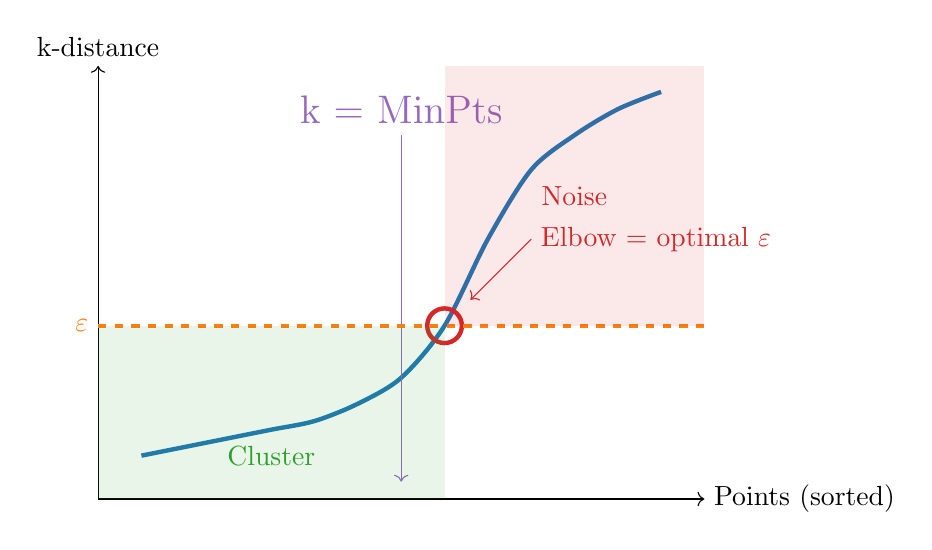
\begin{tikzpicture}[scale=1.1]
% k-distance plot
\draw[->] (0,0) -- (7,0) node[right] {Points (sorted)};
\draw[->] (0,0) -- (0,5) node[above] {k-distance};

% The curve
\draw[mlblue, ultra thick] plot[smooth] coordinates {(0.5,0.5) (1,0.6) (1.5,0.7) (2,0.8) (2.5,0.9) (3,1.1) (3.5,1.4) (4,2) (4.5,3) (5,3.8) (5.5,4.2) (6,4.5) (6.5,4.7)};

% Elbow point
\draw[mlred, ultra thick] (4,2) circle (0.2);
\draw[mlred, <-] (4.3,2.3) -- (5,3) node[right] {Elbow = optimal $\varepsilon$};

% MinPts annotation
\node[mlpurple] at (3.5,4.5) {\Large k = MinPts};
\draw[mlpurple, ->] (3.5,4.2) -- (3.5,0.2);

% eps line
\draw[mlorange, ultra thick, dashed] (0,2) -- (7,2);
\node[mlorange, left] at (0,2) {$\varepsilon$};

% Regions
\fill[mlgreen, opacity=0.1] (0,0) rectangle (4,2);
\fill[mlred, opacity=0.1] (4,2) rectangle (7,5);
\node[mlgreen] at (2,0.5) {Cluster};
\node[mlred] at (5.5,3.5) {Noise};
\end{tikzpicture}
\end{center}

\vspace{1em}

\section*{Discovery Challenge: Optimal Parameters}

\begin{center}
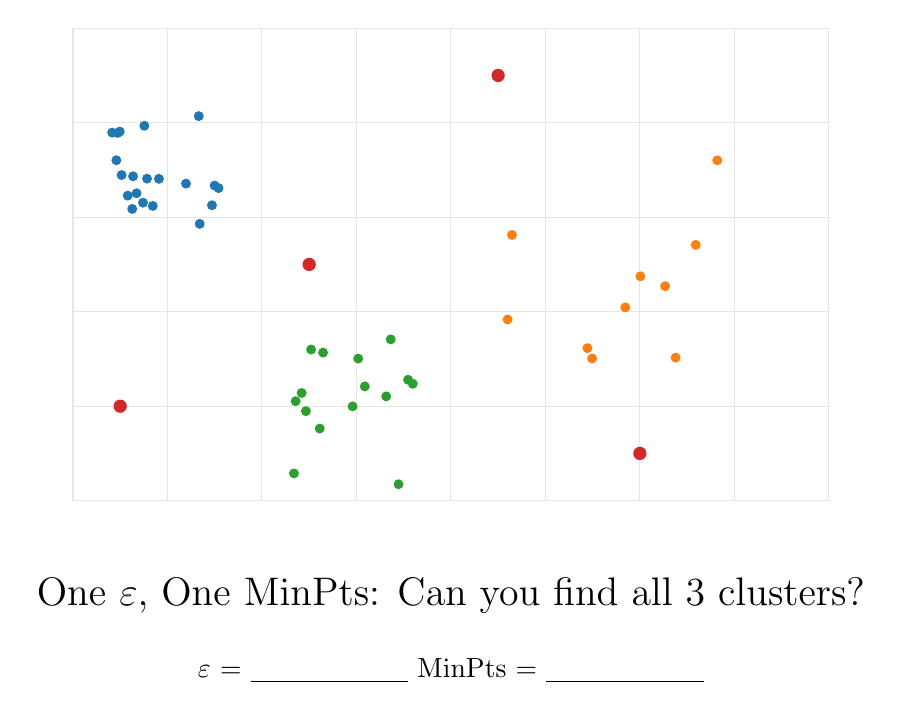
\begin{tikzpicture}[scale=1.2]
% Dataset with varying densities
\draw[gray!20] (0,0) grid (8,5);

% Dense cluster 1
\foreach \i in {1,...,20} {
    \pgfmathsetmacro{\x}{1 + rand*0.6}
    \pgfmathsetmacro{\y}{3.5 + rand*0.6}
    \fill[mlblue] (\x,\y) circle (1.5pt);
}

% Medium cluster 2
\foreach \i in {1,...,15} {
    \pgfmathsetmacro{\x}{3 + rand*0.9}
    \pgfmathsetmacro{\y}{1 + rand*0.9}
    \fill[mlgreen] (\x,\y) circle (1.5pt);
}

% Sparse cluster 3
\foreach \i in {1,...,10} {
    \pgfmathsetmacro{\x}{5.5 + rand*1.5}
    \pgfmathsetmacro{\y}{3 + rand*1.5}
    \fill[mlorange] (\x,\y) circle (1.5pt);
}

% Some noise
\fill[mlred] (2.5,2.5) circle (2pt);
\fill[mlred] (4.5,4.5) circle (2pt);
\fill[mlred] (6,0.5) circle (2pt);
\fill[mlred] (0.5,1) circle (2pt);

\node[font=\Large] at (4,-1) {One $\varepsilon$, One MinPts: Can you find all 3 clusters?};
\node at (4,-1.8) {$\varepsilon$ = \underline{\hspace{2cm}} MinPts = \underline{\hspace{2cm}}};
\end{tikzpicture}
\end{center}

\vspace{0.5em}

\begin{tcolorbox}[colback=mlcyan!10, colframe=mlcyan!50]
\centering\large
\textbf{Next: Hierarchical} - When you need clusters at every scale!
\end{tcolorbox}

\end{document}